
%----------------------------------------------------------------------------------------
%	PACKAGES AND OTHER DOCUMENT CONFIGURATIONS
%---------------------------------------------------------------------------------------

\documentclass[11pt]{scrartcl} % Font size
\newcommand{\comment}[1]{}
%%%%%%%%%%%%%%%%%%%%%%%%%%%%%%%%%%%%%%%%%
% Wenneker Assignment
% Structure Specification File
% Version 2.0 (12/1/2019)
%
% This template originates from:
% http://www.LaTeXTemplates.com
%
% Authors:
% Vel (vel@LaTeXTemplates.com)
% Frits Wenneker
%
% License:
% CC BY-NC-SA 3.0 (http://creativecommons.org/licenses/by-nc-sa/3.0/)
% 
%%%%%%%%%%%%%%%%%%%%%%%%%%%%%%%%%%%%%%%%%

%----------------------------------------------------------------------------------------
%	PACKAGES AND OTHER DOCUMENT CONFIGURATIONS
%----------------------------------------------------------------------------------------

\usepackage{amsmath, amsfonts, amsthm} % Math packages

\usepackage{listings} % Code listings, with syntax highlighting

\usepackage[english]{babel} % English language hyphenation

\usepackage{graphicx} % Required for inserting images
\graphicspath{{Figures/}{./}} % Specifies where to look for included images (trailing slash required)

\usepackage{booktabs} % Required for better horizontal rules in tables

\numberwithin{equation}{section} % Number equations within sections (i.e. 1.1, 1.2, 2.1, 2.2 instead of 1, 2, 3, 4)
\numberwithin{figure}{section} % Number figures within sections (i.e. 1.1, 1.2, 2.1, 2.2 instead of 1, 2, 3, 4)
\numberwithin{table}{section} % Number tables within sections (i.e. 1.1, 1.2, 2.1, 2.2 instead of 1, 2, 3, 4)

\setlength\parindent{0pt} % Removes all indentation from paragraphs

\usepackage{enumitem} % Required for list customisation
\setlist{noitemsep} % No spacing between list items

%----------------------------------------------------------------------------------------
%	DOCUMENT MARGINS
%----------------------------------------------------------------------------------------

\usepackage{geometry} % Required for adjusting page dimensions and margins

\geometry{
	paper=a4paper, % Paper size, change to letterpaper for US letter size
	top=2.5cm, % Top margin
	bottom=3cm, % Bottom margin
	left=3cm, % Left margin
	right=3cm, % Right margin
	headheight=0.75cm, % Header height
	footskip=1.5cm, % Space from the bottom margin to the baseline of the footer
	headsep=0.75cm, % Space from the top margin to the baseline of the header
	%showframe, % Uncomment to show how the type block is set on the page
}

%----------------------------------------------------------------------------------------
%	FONTS
%----------------------------------------------------------------------------------------

\usepackage[utf8]{inputenc} % Required for inputting international characters
\usepackage[T1]{fontenc} % Use 8-bit encoding

\usepackage{fourier} % Use the Adobe Utopia font for the document

%----------------------------------------------------------------------------------------
%	SECTION TITLES
%----------------------------------------------------------------------------------------

\usepackage{sectsty} % Allows customising section commands

\sectionfont{\vspace{6pt}\centering\normalfont\scshape} % \section{} styling
\subsectionfont{\normalfont\bfseries} % \subsection{} styling
\subsubsectionfont{\normalfont\itshape} % \subsubsection{} styling
\paragraphfont{\normalfont\scshape} % \paragraph{} styling

%----------------------------------------------------------------------------------------
%	HEADERS AND FOOTERS
%----------------------------------------------------------------------------------------

\usepackage{scrlayer-scrpage} % Required for customising headers and footers

\ohead*{} % Right header
\ihead*{} % Left header
\chead*{} % Centre header

\ofoot*{} % Right footer
\ifoot*{} % Left footer
\cfoot*{\pagemark} % Centre footer
 % Include the file specifying the document structure and custom commands
%\usepackage{flafter}
\usepackage[section]{placeins}
\usepackage{caption}
\usepackage{float}
%----------------------------------------------------------------------------------------
%	TITLE SECTION
%----------------------------------------------------------------------------------------

\title{	
	\normalfont\normalsize
	\textsc{Rutgers University, New Brunswick}\\ % Your university, school and/or department name(s)
	\vspace{25pt} % Whitespace
	\rule{\linewidth}{0.5pt}\\ % Thin top horizontal rule
	\vspace{20pt} % Whitespace
	{\huge Mazes}\\ % The assignment title
	\vspace{12pt} % Whitespace
	\rule{\linewidth}{2pt}\\ % Thick bottom horizontal rule
	\vspace{12pt} % Whitespace
}

\author{\LARGE Eshaan Gandhi, Siddarth Mandayam} % Your name

\date{\normalsize\today} % Today's date (\today) or a custom date

\begin{document}

\maketitle % Print the title

\section{The maze is on fire}

\subsection{Testing out our environment}
What I mean by testing out our environment is that we wanted to demonstrate the maze being generated with a given block density $\rho$. We also wanted to demonstrate the placement of fire and initial path to the target.\\

So we first generated a few maps with varying levels of block-density as demonstrated by the graphics below. \\
\begin{figure}[H]
 	\begin{center}
 	\includegraphics*[scale=0.3]{GUI3C.png}
	\caption{The map that is generated for p=0.3}
	\label{fig:example}
	
 	\end{center}
 
 \end{figure}
	\begin{figure}[H]
 	\begin{center}
	\includegraphics*[scale=0.3]{GUI4C.png}
	\caption{The map that is generated for p=0.6}
	\label{fig:example}
	\vspace{2em}
	\includegraphics*[scale=0.3]{GUI5C.png}
	\caption{The map that is generated for p=0.9}
	\label{fig:example}
	\end{center}
	\end{figure}
%Add image of the empty mazes
\pagebreak
Next we would like to confirm that one element at random gets set on fire and spreads as demonstrated by the graphics below. \\

\begin{figure}[H]
 	\begin{center}
 	\includegraphics*[scale=0.3]{GUI6C.png}
	\caption{The map fire being placed}
	\label{fig:example}
	\vspace{2em}
	\includegraphics*[scale=0.3]{GUI7C.png}
	\caption{The fire spreading after a few turns}
	\label{fig:example}
	
 	\end{center}
  	
	
 \end{figure}

%add image of fire and fire spreadying for flammability q

\subsection{Strategy 1}
So strategy 1 is a naive way to go about this, but would not require that many resources to go about it. It simply does not care about the fire, and the person does get burned pretty often. Here is the strategy statement in detail. At the start of the maze, wherever the fire is, we solve for the shortest path from upper left to lower right, and follow  it  until the  agent  exits  the  maze  or  burns.   This  strategy  does  not  modify  its  initial  path  as  the  fire changes.
\vspace{2em}\\
We were tasked in generating a plot of ‘average successes vs flammability $q$’. To do that we had to run our program for strategy 1 $n$ number of times. In the assignment document, the minimum number is 10, but we realized that these many tries does not represent the true statistic well because of variance. So we in turn ran the maze a 1000 times for 11 values of q - 0 .. 1. \\
We have recorded our finding in the table above.\\
\begin{table}[!htb]
\caption{Strategy 1}
\begin{tabular}{|l|l|l|l|}
\hline
\textbf{Valid iterations} & \textbf{q - flammability rate} & \textbf{s - successes} & \textbf{u - Times the agent got burned} \\ \hline
1000 & 0.0   & 736 & 264 \\ \hline
1000 & 0.1 & 556 & 444 \\ \hline
1000 & 0.2 & 375 & 625 \\ \hline
1000 & 0.3 & 316 & 684 \\ \hline
1000 & 0.4 & 181 & 819 \\ \hline
1000 & 0.5 & 162 & 838 \\ \hline
1000 & 0.6 & 95  & 905 \\ \hline
1000 & 0.7 & 75  & 925 \\ \hline
1000 & 0.8 & 59  & 941 \\ \hline
1000 & 0.9 & 42  & 958 \\ \hline
1000 & 1.0   & 37  & 963 \\ \hline
\end{tabular}
\end{table}

\begin{figure}[H]
 	
  	\includegraphics*[scale=0.8]{strategy1.png}
	%\caption{Recursion tree and analysis}
	\label{fig:example}
 \end{figure}

\subsection{Strategy 2}
So strategy 2 is a better way to go about this than strategy 1, but would require more resources than strategy 1. It recomputes it's path every time it makes a step. Here is the strategy statement in detail. At every time step, we re-compute the shortest path from the agent’s current position to the goal position, based on  the  current  state  of  the  maze  and  the  fire.  We then follow  this  new  path  one  time  step,  then  re-compute.   This strategy constantly re-adjusts its plan based on the evolution of the fire.  If the agent gets trapped with no path to the goal, it dies.
\vspace{2em}\\
We were tasked in generating a plot of ‘average successes vs flammability $q$’. To do that we had to run our program for strategy 2 $n$ number of times. In the assignment document, the minimum number is 10, but we realized that these many tries does not represent the true statistic well because of variance. So we in turn ran the maze a 1000 times for 11 values of q - 0 .. 1.\vspace{2em}\\
We have recorded our finding in the table above.\\
\begin{table}[!htb]
\begin{tabular}{|l|l|l|l|}
\hline
\textbf{Valid iterations} & \textbf{q - flammability rate} & \textbf{s - successes} & \textbf{u - Times the agent got burned} \\ \hline
1000 & 0.0   & 913 & 87  \\ \hline
1000 & 0.1 & 706 & 294 \\ \hline
1000 & 0.2 & 451 & 549 \\ \hline
1000 & 0.3 & 353 & 647 \\ \hline
1000 & 0.4 & 241 & 759 \\ \hline
1000 & 0.5 & 172 & 828 \\ \hline
1000 & 0.6 & 134 & 886 \\ \hline
1000 & 0.7 & 70  & 930 \\ \hline
1000 & 0.8 & 68  & 932 \\ \hline
1000 & 0.9 & 46  & 954 \\ \hline
1000 & 1.0 & 52  & 948 \\ \hline
\end{tabular}
\end{table}\\
\begin{figure}[H]
 	\centering
  	\includegraphics*[scale=0.8]{strategy2.png}
	%\caption{Recursion tree and analysis}
	\label{fig:example}
 \end{figure}

\subsubsection{This is our analysis for the 2nd strategy.}
We can see that this strategy is much more effective than the 1st one, but at the same time is way more computationally expensive. We are running a $O(b^d)$ algorithm with a branching factor of 4 $k$ number of times. If you think about if a "intelligent being" was in the maze, they would not be able to compute the solution in time. 

\subsection{Strategy 3 - GTFO! (Graph The Fire Out)}
We then wanted to try out our own strategy. The problem with strategy 1 and strategy 2 is that it does not take into consideration changing state of the maze and future state of the maze respectively. So we thought we could simulate part of the maze and see how we do. We started out simulating the whole maze but that would just mean that the fire engulfs the whole maze and finding a path is near impossible. So we simulate a part of the maze and try to find a path. We then take that path in the original maze and would likely make it. If we do make it, then we simulate it again. This strategy takes the future states into account, moves a bit, and then takes into account the changing state of the fire. \vspace{2em}\\

Well we found out it does very well for when the fire is not spreading rapidly, but does rather poorly when the fire is pretty fast. Here is the data.\\

%\begin{figure}[H]
\begin{table}[!htb]
\begin{tabular}{|l|l|l|l|}
\hline
\textbf{Valid iterations} & \textbf{q - flammability rate} & \textbf{s - successes} & \textbf{u - Times the agent got burned} \\ \hline
1000 & 0.0   & 919 & 81  \\ \hline
1000 & 0.1 & 651 & 349 \\ \hline
1000 & 0.2 & 453 & 547 \\ \hline
1000 & 0.3 & 337 & 663 \\ \hline
1000 & 0.4 & 214 & 786 \\ \hline
1000 & 0.5 & 159 & 841 \\ \hline
1000 & 0.6 & 99  & 901 \\ \hline
1000 & 0.7 & 74  & 926 \\ \hline
1000 & 0.8 & 54  & 946 \\ \hline
1000 & 0.9 & 58  & 942 \\ \hline
1000 & 1.0   & 39  & 961 \\ \hline
\end{tabular}
\end{table}

\begin{figure}[H]
 	\centering
  	\includegraphics*[scale=0.8]{strategy3.png}
	%\caption{Recursion tree and analysis}
	\label{fig:example}
 \end{figure}


%\end{figure}
%Note - We use a numpy 2-d array to represent our maze and this should be well documented in our code. \\
\paragraph{Extra Credit}
Do we get it? GTFO is the acronym. 
\subsection{Comparison}
If we look at all the data, we can conclude that strategy 2 might be the best strategy, but it is very computationally expensive. We calculate the BFS path at every step. Our player might not have that kind of time when the fire is spreading fast.\vspace{2em}\\
For the first strategy the time complexity is $O(b^{d+1})$ as we only compute BFS once. Where $b = 4$ as we are computing 4 adjacent nodes.\vspace{2em}\\
Now if we look at Strategy 2, we are doing BFS on every movement. That is $O(k(b^{d+1})$ In real time we probably don't have that much time to make a decision in a maze that may be burning pretty fast.\vspace{2em}\\
The third strategy is simulating the future fire. If we were in a maze, we could kind of eyeball what the fire would look like. Simulating fire is not that computationally heavy and we only have to do BFS a fraction of the time we do it in strategy 2. We also get very similar results if we go about strategy 3. 



\subsection{Note on dimensions}
As we mentioned the time complexities of all three methods, this becomes very computationally expensive for the computer. I also wanted to generate a lot more maps than 10 as that removes variance. There are a number of times when we generate a map and it is rejected as there is not even an initial way to the goal. For these reasons, I chose a non-trivial dimension that is fast enough to run more than 1000 times for each value of $q$ and also large enough for the maze solve not to be trivial. 

\pagebreak
\section{Maze Thinning}

\subsection{Testing out our environment}
In the maze thinning part of the project, we are still using the same maze environment as the one in the previous part. We still generate a maze with a given block density of $p$, however this time, there is no fire. While we used Breadth-First Search (BFS) in the previous part, in this part we aim to use the A* search algorithm to find a way through the maze. The benefits to A* is that if we choose a consistent heuristic, we can find the most optimal path (if there is one) through the maze while also expanding fewer nodes through our search than BFS.\vspace{2em}\\
We want to demonstrate out thinning maze function works and hence we generated these images. 
\begin{figure}[H]
 	\centering
  	\includegraphics*[scale=0.3]{Maze.png}
	\caption{Maze before thinning}
	\label{fig:example}
 \end{figure}
 \begin{figure}[H]
 	\centering
  	\includegraphics*[scale=0.3]{MazeThinned.png}
	\caption{Maze after thinning}
	\label{fig:example}
 \end{figure}
\subsection{Strategy 1 - A* Manhattan}

There are several means of generating heuristics. Our first strategy generates heuristics using Manhattan Distance, which estimates the distance a node is from the goal by adding up its vertical and horizontal distance, or some would call it - the Manhattan Distance (w/o Broadway).\vspace{2em}\\
This heuristic is best for using in mazes where one can only move left, right, up, or down, similar to how one could only move left, right, up or down streets in Manhattan. Manhattan Distance is also a consistent heuristic because the estimated cost of reaching the goal from a node $n$ is no worse than the estimated cost of going to the goal from $n$ through a child of $n'$, a child of $n$. This is because we are restricted to only moving up, down, left, or right, and we are moving along a grid that is unweighted, where each step cost to move from one square to another is the same. We also know that if Manhattan Distance is consistent, then Manhattan Distance is also an admissible heuristic, meaning it does not overestimate the true or optimal cost of reaching the goal node. This is because you can only move in four directions, and it calculates the vertical and horizontal distances without taking into account blocked squares that might be in the way. 

\subsection{Strategy 2 - Thin Maze Shortest Path Lengths}

Manhattan Distance is an example of a geometric heuristic where we use distance as a means of calculating heuristics. Another means is known as relaxations, where we solve simpler versions of the problem. \vspace{2em}\\
One such relaxation is thinning the maze by removing a certain proportion $\rho$ of the blocked squares from the maze. With this easier to solve thinned map, we can use A*-Manhattan to calculate the shortest path to the goal from each square and use that as a heuristic for the original map. This method is consistent because we are using shortest paths lengths derived from running A* Manhattan on the thinned maze. And because we are using shortest path lengths from the thinned maze, which is easier to solve, we essentially create a lower bound on the distance to the goal in the original maze.

\subsection{Strategy 3 - BFS Diagonal} 

One relaxation we thought we could use is to calculate an optimal path for each cell using BFS in the thinned maze, but this time, we can move diagonally. We then use the length of the path as a heuristic. The reason we chose to do this is because in an earlier lecture, when talking about generating heuristics through relaxations, we discussed that one way of doing so was by giving yourself "superpowers" in which you could allow yourself more flexibility and have less restrictions on what you are allowed to do in order to reach the goal state. For example, we discussed a sliding tile game where we have a 3 by 3 grid with one square empty and the rest of the numbers randomly placed. The goal of the game was to make the least amount of moves to get the board from the initial state to the goal state as seen below.

\begin{figure}[H]
  	\centering
  	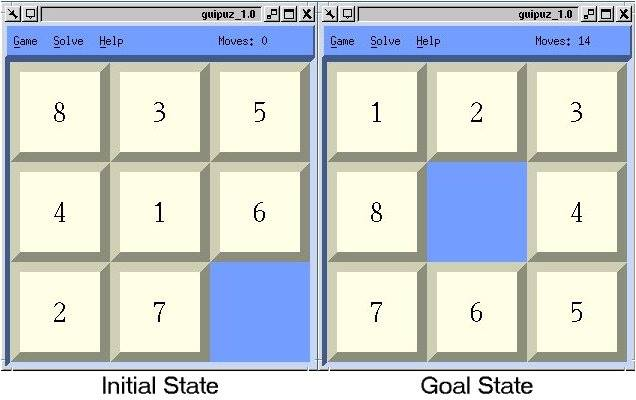
\includegraphics[scale=0.3]{class.jpg}
	\caption{Picture of relaxation - taken from class}
	\label{fig:example}
  \end{figure}
 
 \vspace{2em}

In class we talked about how one way we could go about using a relaxation to getting a heuristic function for this problem is that we could say that we have the power to simply swap numbers from their positions. For example, starting with the initial state shown above, we swap 1 with 8, 2 with 3, 3 with 5, and so on. Obviously, we can only move numbers to the empty space instead of swap, but by introducing this "superpower" of swapping, we can establish a lower bound on the number of moves needed to reach the goal state, thus creating a heuristic.

\vspace{2em}
For the maze problem, we decided to use the "superpower" of moving diagonally with regards to finding the most optimal path via BFS. If a position that is closer to the goal is a diagonal away from where we are currently, we can simply move there in one move as opposed to having to 1 vertical and 1 horizontal move to get there. Thus we set a lower bound on the number of moves we can make which we can use as a heuristic.

\vspace{2em}

\subsection{Comparison}
For each strategy, we kept the obstacle density the same at $p = 0.3$. We then ran and solved 1000 mazes each strategy, for each $\rho$ that would be used to thin the maze. We also generated 10 by 10 mazes to test each strategy as this was the largest sized maze that we could run repeatedly for such a large amount of mazes and finish in a reasonable time. We also did not count any mazes were there is no path to the goal. We recorded our findings in the table above.
\begin{center}

\begin{table}[H]
\begin{tabular}{|l|l|l|l|l|}

\hline
\textbf{Valid iterations} & \textbf{$\rho$} & \textbf{Strategy 1} & \textbf{Strategy 2} & \textbf{Strategy 3}	\\ \hline
1000 & 0.0 & 0.536 & 0.440 & 0.576 \\ \hline
1000 & 0.1 & 0.542 & 0.466 & 0.571 \\ \hline
1000 & 0.2 & 0.535 & 0.474 & 0.578 \\ \hline
1000 & 0.3 & 0.542 & 0.499 & 0.577 \\ \hline
1000 & 0.4 & 0.539 & 0.506 & 0.571 \\ \hline
1000 & 0.5 & 0.541 & 0.520 & 0.573 \\ \hline
1000 & 0.6 & 0.536 & 0.521 & 0.575 \\ \hline
1000 & 0.7 & 0.538 & 0.529 & 0.574 \\ \hline
1000 & 0.8 & 0.536 & 0.531 & 0.572 \\ \hline
1000 & 0.9 & 0.537 & 0.535 & 0.578 \\ \hline
1000 & 1.0 & 0.538 & 0.538 & 0.579 \\ \hline
\end{tabular}
\caption{Average Fraction of Nodes Expanded for each Strategy}
\end{table}

\begin{figure}[H]
 	\centering
  	\includegraphics*[scale=0.8]{line-graph-4.png}
	%\caption{Recursion tree and analysis}
	\label{fig:example}
 \end{figure}

\end{center}
Strategy 1 just consists of doing A*-Manhattan over the original maze. No thinning is involved, so $\rho$'s value is irrelevant to Strategy 1. Nonetheless, we see that Strategy 1 on average expands 53.8 percent of the total nodes in the maze when finding the optimal solution.

\vspace{1em}

When we examine Strategy 2, we see that as $\rho$ increases the average percentage of total nodes expanded increases. The lowest total percentage is found when $\rho = 0$ at 44 percent. However, we want to disregard this because what is essentially happening when $\rho = 0$ is that we are just running A*-Manhattan on the original maze, and using the shortest path lengths generated as a heuristic. We are not using relaxations to make estimates on the lower bound of moves needed to reach the goal.

\vspace{1em}

We see that for $\rho = 0.1$, $\rho = 0.2$, $\rho = 0.3$, and $\rho = 0.4$, the difference between the average percentage of nodes expanded for Strategy 1 and Strategy 2 are very noticeable. From this data, we can conclude that when we thin a small percentage of the maze, we can significantly reduce the amount of lookups needed to find the goal by using A*-Manhattan to gather shortest length paths from the thinned maze.\vspace{2em} \\
However, around $\rho = 0.5$, we can see from the table and graph that as $\rho$ increases from this point, we move closer to the amount of lookups needed in Strategy 1. However, we can conclude from this data that values of 0.1, 0.2, 0.3, and 0.4 for $\rho$ help make the maze thinning strategy a viable option. However, time costs to be aware of is that we are using A*-Manhattan for every single node we encounter in order to generate heuristics.

\vspace{1em}

Looking at Strategy 3, we see that it performs worse than both Strategy 1 and Strategy 2 when it comes to lookups, with an average of 57.5 percent of nodes explored. After observing this, we believe that the reason it performs worse than the other 2 strategies because it is not a consistent heuristic like the other 2 strategies. The reason being, we are allowing our BFS to also search diagonal neighbors, which gives us a lower bound of moves. However, it does not work as well in the actual maze where we are not allowed to move diagonal, but only in cardinal directions. We learned from this that when you are only allowed to move in specific directions, expanding the directions you can move in to determine your heuristics may give a lower bound of moves, but it does not correlate well to actual execution. Thus, we concluded that Strategy 3 is not a viable option compared to the other 2 strategies.


\end{document}